\documentclass[msc, cs, deptreport, singlespacing, twoside]{infthesis}
\usepackage{listings}
\usepackage{color}
\usepackage{geometry}
\usepackage{graphicx}
\usepackage{float}
\usepackage{subfig}
\usepackage{array}
\usepackage{textcomp}
\usepackage[colorlinks=true, citecolor=black, linkcolor=black, urlcolor=black, bookmarks]{hyperref}
 
\definecolor{javared}{rgb}{0.6,0,0} % for strings
\definecolor{javagreen}{rgb}{0.25,0.5,0.35} % comments
\definecolor{javapurple}{rgb}{0.5,0,0.35} % keywords
\definecolor{javadocblue}{rgb}{0.25,0.35,0.75} % javadoc

\lstset{
	language=Java,
	basicstyle=\footnotesize\ttfamily,
	keywordstyle=\color{javapurple}\bfseries,
	stringstyle=\color{javared},
	commentstyle=\color{javagreen},
	morecomment=[s][\color{javadocblue}]{/**}{*/},
	numbers=left,
	frame=single,
	numberstyle=\tiny\color{black},
	stepnumber=1,
	numbersep=10pt,
	tabsize=2,
	showspaces=false,
	showstringspaces=false
}


\title{Radio Frequency Localisation/Tracking of RFID Tags in a Raspberry-Pi Sensor Network}
\author{Aleksandar Krastev}

\abstract{
To Do
}

\begin{document}
\begin{preliminary}
\maketitle
\begin{acknowledgements}
To Do
\end{acknowledgements}
\standarddeclaration
\tableofcontents
\end{preliminary}

\chapter{Introduction}
\label{ch:introduction}

Radio frequency identification (RFID) is a technology that enables the recognition of objects tagged with an RFID transmitter. It functions by remotely obtaining data stored on RFID tags. This information is mainly used for identification purposes. Systems relying on such data can only provide course-grained location information \cite{Bouet2008}. Their RFID readers are positioned at strategic control points that sense tags entering their read range. However, if an object's identity is combined with its location, then the benefits of RFID could be greater. For example, patient care and hospital operations could be improved using remote identification and tracking of patients \cite{Cangialosi2007}. Also, the attendance of children at schools could be monitored \cite{Swartz2004}.

RFID localisation principles are similar to the ones used for indoor wireless networks \cite{Bouet2008}. There are certain differences between both technologies, which results in tracking methods that are altered to reflect the characteristics of RFID. This project uses the trilateration localisation technique to determine the position of a tag using three reader nodes in a controlled indoor environment.

RFID systems consist of tags and readers. While tags are simple devices, readers are more complex and usually require a connection to a host computer or network \cite{Landt2005}. The high costs of tags and readers are a major factor that constrains the penetration of this technology \cite{Want2006}. Nowadays, these devices are becoming affordable to users. In addition, the recent emergence of cheap and compact single-board computers, such as the Raspberry Pi\footnote{About the Raspberry Pi - \url{http://www.raspberrypi.org/about}}, creates an exiting opportunity to build a cost-effective RFID sensor network capable of localising tags. This can be realised by connecting readers to single-board computers to obtain the identity of tags and a measure of the signal strength, which could provide an estimation of the distance between receivers and transmitters.

On the one hand, the RFID technology has unprecedented advantages and it has gained the attention of big industries that have identified its potential \cite[p. 39]{Hunt2007}. On the other hand, the high costs of RFID tracking systems and components prevent most people from using and developing the technology\footnote{How much do RFID readers cost today? - \url{http://www.rfidjournal.com/faq/show?86}}. The hardware combination of affordable readers, tags, and single-board computers has the potential to benefit a vast range of businesses, but also do-it-yourself hobbyists and enthusiasts. This might result into improved automated handling and tracking of goods in a warehouse, for instance. It can also result in a fast-paced open-source development of the RFID technology applied in a wide range of scenarios. Constructing such a system is exiting because it can show that there can be cost-effective alternatives to commercial solutions, thus making the technology accessible to a wider audience.

\section{Hypothesis}

The hypothesis of this project is that existing localisation techniques can be applied to a cost-effective Raspberry-Pi sensor network to build a location sensing system achieving a localisation accuracy comparable to existing approaches. More specifically, the purpose of the project is to construct and programme three reader nodes, each consisting of an RFID reader connected to a single-board computer, cooperating in an indoor environment to estimate the position of a stationary or moving active tag based on the received signal strength indicator (RSSI) provided by the readers. This metric is converted to distance used by the trilateration geometrical process to compute the position of an unknown object.

\section{Results}

The above system was developed during the course of this project. A number of experiments measured the system's performance in terms of localisation error between the real and estimated positions of the tag. The average location error from these tests was 0.916 meters on each side of the object. These results are similar to the achievements of the previous work in this research field. Although the system could be tested in more scenarios under different conditions, these results confirmed that an affordable RFID positioning system can be built and operate with a reasonable performance.

\section{Thesis Outline}

This document consists of six chapters. The organisation is as follows:
\begin{itemize}
\item \textbf{Chapter \ref{ch:background}} gives background information on radio frequency identification, the hardware and  localisation algorithm used in this project. In addition, this chapter provides a literature review of previous work in this research field.
\item \textbf{Chapter \ref{ch:methodology}} describes an overview of the hardware setup of the system. In addition, it contains a definition of the problem this project is trying to solve. The rest of the chapter presents the overall design of the system and the methods for converting received signal strength indicator to distance. The trilateration geometrical process used to estimate the position of the tag is also described.
\item \textbf{Chapter \ref{ch:implementation}} gives implementation details of all parts of the system. This chapter lists the software engineering practices that helped to develop the system. Any implementation difficulties are also discussed.
\item \textbf{Chapter \ref{ch:evaluation}} contains experiments that test the RFID hardware. In addition, the performance of the system is investigated and measured. The chapter includes a discussion, where results are compared with achievements of previous projects.
\item \textbf{Chapter \ref{ch:conclusion}} concludes this work by presenting the contributions of this project and suggesting future directions in which the system can be extended.
\end{itemize}

\section{Summary}

This chapter provided the motivation for this project. It also defined the hypothesis that is checked in this work. The main results were also given. Finally, the structure of this document was described. The next chapter provides background information on the technology and hardware used in this project. In addition, the previous work in this field is summarised.

\chapter{Background}
\label{ch:background}

This chapter presents background information of the technologies and hardware used in this project. First, an introduction of RFID is provided in Section \ref{sec:rfid}. This includes a description of the technology, typical components of such systems, and potential applications in the context of this work. Then, Section \ref{sec:rssi} discusses the Received Signal Strength Indicator (RSSI) as the metric for measuring distance between readers and tags. Next, the hardware components of the project are presented in Section \ref{sec:projhard}. These are RFID readers, an active tag, and single-board computers (Raspberry Pis). Section \ref{sec:locsens} includes a discussion of location sensing techniques and evaluation criteria used throughout this project. This chapter is concluded by a survey of previous work using active RFID components to localise objects in indoor environments.

\section{Radio Frequency Identification (RFID)}
\label{sec:rfid}

Radio Frequency Identification (RFID) is a wireless technology that communicates electronically stored data between radio devices. This information is used to remotely identify objects marked with tags \cite[p. 5]{Hunt2007}. RFID uses electromagnetic waves to carry information. Such systems differ from each other by their radio frequency of operation, physical coupling method, and transmission range \cite[p. 21]{Finkenzeller2010}. Radio frequencies used in RFID range from 100kHz to 10GHz \cite{Landt2005}. The physical coupling methods in RFID classify such systems into three main categories. Close-coupling systems have a small interrogation range of up to 1cm. Remote coupled systems are capable of sensing information of up to 1m. All systems that can wirelessly read data from a marked object positioned over 1m away are called long-range systems \cite[p. 22]{Finkenzeller2010}. An RFID system has three compulsory hardware components, tags (also known as transpoders), readers (also called interrogators), and controllers.

\subsection{RFID tags}

A tag is a data-carrying device that transmits identification information in response to a received signal from a reader. RFID tags usually consist of an antenna attached to a microchip \cite[p. 2]{Want2006}. The hardware can be encapsulated in different types of enclosures. Tags come in different shapes and sizes depending on their operational environment (Figure \ref{fig:rfidtags}). RFID tags also have memory where the identification and sometimes additional information is stored. Additional data might include a delivery date of a parcel, for example. The information stored on a tag is usually only for reading. However, there are implementations of the RFID technology that benefit from writing data to a tag. For instance, a pallet might have a tag attached to it that can store the content of the pallet as it changes over time \cite[p. 8]{Hunt2007}.

\begin{figure}
	\begin{center}
		\includegraphics[width=0.5\textwidth]{figures/rfidtags}
		\caption{Three different variants of RFID tags. Figure from \cite{Want2006}.}
		\label{fig:rfidtags}
	\end{center}
\end{figure}

\subsubsection{Passive and active tags}

Tags can be classified into two main categories, passive and active. Passive tags do not require a power source. They communicate with readers by reflecting part of received radio waves, a term referred to as backscatter modulation \cite{Bolic2010}. They have a number of advantages, which include their small size, very long operational life, and low price. Nevertheless, passive tags need to be in the readers' range in order to operate. This is because passive tags obtain the power they need to supply their circuitry from an electromagnetic signal received from an RFID reader. A charge builds up into a capacitor that can power the passive tag and transmit the identification information it is storing \cite{Weinstein2005}.

In contrast, active tags require a power source in the form of a battery or are directly connected to the electrical grid \cite{Want2006}. Although their lifetime might be limited by the available energy, active tags can be read from greater distances compared to passive tags. This is because they have their own power source which enables them to emit strong signals to the readers \cite{Weinstein2005}. Compared to passive tags, active ones are larger in size and have a higher price.

\subsection{RFID readers}

A reader is a radio device that is capable of transmitting interrogation signals and capturing information send back by tags. The reader's transmission frequency specifies the operational frequency of the RFID system, which also defines their practical reading range \cite{Finkenzeller2010}. These devices usually consist of a radio frequency (RF) module that is capable of sending and receiving  signals, an antenna, and a control unit in the form of a microprocessor. RFID readers have the following main functions:

\begin{itemize}
	\item read/write data from/to an RFID tag,
	\item power a passive tag,
	\item relay the obtained information to a host computer \cite[p. 9]{Hunt2007}.
\end{itemize}

Readers are responsible for bringing additional functionality to an RFID system. This includes support for simultaneous sensing of multiple tags, authentication of tags to prevent unauthorised access to a system, and data encryption of the stored data to ensure integrity \cite[p. 10]{Hunt2007}. There is a wide range of RFID readers that differ in their operational radio frequency, range, and coupling method. These properties are formed by factors such as the specifications of the system, its budget, and security requirements \cite[p. 25]{Finkenzeller2010}.

\subsection{RFID controllers}

The third component of an RFID system is the controller or server. It is a computer that is responsible for connecting and communicating with multiple readers, aggregating any incoming data, and processing it. Readers can be connected to the server using a network or serial connection. Identification information is usually stored in a database and is used by an application software \cite[p. 11]{Hunt2007}. Figure \ref{fig:rfidsys} shows the components of a typical RFID system.

\begin{figure}[h]
	\begin{center}
		\includegraphics[width=0.5\textwidth]{figures/rfidsys}
		\caption{Components and applications of RFID. Figure from \cite[p. 20]{Rida2010}.}
		\label{fig:rfidsys}
	\end{center}
\end{figure}

\subsection{RFID applications}

RFID hardware is becoming more inexpensive, which creates a wide range of possible scenarios where this technology can be applied \cite{Nath2006}. The most widespread applications are in tracking of objects or people, in supply chain and asset management, and in health services \cite{Weinstein2005}.

Passive RFID systems can be used as an alternative and improvement of the current standard for identification of products, the barcodes.  Reading a barcode attached to an object requires a direct line of sight between a reader and a tag. In addition, barcodes can get obscured by other objects or substances, which hinders the identification process. RFID solves these disadvantages. A line of sight is not required when reading data from tags attached to objects. RFID tags also support a larger set of unique IDs compared to bar codes, can be reprogrammed, and can store additional data depending on the application requirements \cite{Weinstein2005}.

In the context of this project, which is concerned with location sensing, RFID has applications in tracking important objects or personnel and trying to pinpoint their position. For example, active RFID systems can be used in hospitals to monitor the location and life cycle of patients in an indoor environment \cite{Cangialosi2007}. Expensive hospital equipment could be tracked so that it would be at the right place and time. Another possible scenario is to track school kinds while on school grounds in order to find lost children and monitor their attendance \cite{Swartz2004}.

\section{Received Signal Strength Indicator (RSSI)}
\label{sec:rssi}

Some RFID readers provide an indication of the strength of radio signals received from tags. This metric is called Received Signal Strength Indicator (RSSI). Its value is often output along with the identity information stored in a tag. It is estimated at the reader side before amplifying the received input. RSSI is a unitless measurement of the power of the received signal represented as a positive value with certain resolution range. A resolution of three bits gives a precision of eight possible values for RSSI. This means that there are eight different steps of estimating how far a tag is. A resolution of eight bits, supported by the project hardware, lets readers output values between 0 and 255 giving a better approximation of the distance between a reader and a tag. 

\subsection{RSSI and RSS}
\label{subsec:rssiandrss}

RSSI is not to be confused with the Received Signal Strength (RSS), on which RSSI is based. RSS is usually measured in dBm\footnote{dBm - Power ratio in decibels of power referenced to one milliwatt (mW) - \url{http://en.wikipedia.org/wiki/DBm}}. It represents the attenuation of a received signal and is a function of the distance between a receiver and transmitter \cite{Bouet2008}. In WiFi, the 802.11 standard does not define the relationship between RSSI values and reported signal power levels. It is up to the manufacturers to provide a conversion function or table that specifies range and accuracy of the RSS values and how these translate into a RSSI range between zero and a maximum value \cite{Lui2011}. The above applies to RFID, which is also a radio technology. 

\subsection{RSSI and distance}
\label{subsec:rsssianddist}

A third relationship is the one between RSSI and distance. In other words, it is the problem of using RSSI reader measurements to estimate the distance separating a receiver and transmitter. More importantly, one might ask whether RSSI is a reliable parameter for localisation algorithms in wireless networks. This is not the main question that this work is concerned with. However, the reliability of this measure is of prime importance because here position estimation relies solely on this parameter. 

On the one hand, there are studies that test the reliability of both RSS and RSSI for location sensing \cite{Elnahrawy2004, Parameswaran2009}. These concluded that the limitations of determining inter nodal distances are fundamental. On the other hand, signal strength is readily available in devices today, which creates attractive opportunities for estimating position without any additional hardware. Indeed, there are a number of WiFi-based systems that rely on received signal strength including the Horus WLAN location system \cite{Youssef2005}, the EZ localisation system \cite{Chintalapudi2010}, an indoor location system using trilateration \cite{Cook2005}.

\subsection{How RSSI fits in this project}

Although RSSI is not considered a reliable measure for distance due to the physical properties of radio waves and due to cluttered and dynamic indoor environments, the aforementioned systems show that researchers and engineers try to get the best of what already is provided. In the same manner, this work uses RSSI reader measurements as a basis for location sensing. This is done using a translation table that converts RSSI into a distance metric. The methods used and the challenges faced are discussed in Section \ref{sec:rssitodist}.

\section{Project Hardware}
\label{sec:projhard}

This project combines three types of hardware. The first is active RFID devices, the second - single-board computers, and the last is a commodity network infrastructure. The main hardware components can be seen on Figures \ref{fig:projrfid} and \ref{fig:projcomp}. The following subsections present these devices and their specifications. Details on how the components are combined in forming the resulting system are given section \ref{sec:hardset}. 

\begin{figure}[h]
	\begin{subfigure}[b]{0.5\textwidth}
		\includegraphics[width=\textwidth]{figures/readers}
		\caption{Three active RFID readers}
		\label{fig:projread}
	\end{subfigure}
	\begin{subfigure}[b]{0.5\textwidth}
		\includegraphics[width=\textwidth]{figures/tag}
		\caption{One active RFID tag}
		\label{fig:tag}
	\end{subfigure}
	\caption{RFID hardware used in this project.}
	\label{fig:projrfid}
\end{figure}


\subsection{RF9315R-u Active RFID 8 Meters Receiver with RSSI Module}
\label{subsec:receiver}

The project uses three active RFID readers containing RSSI modules. Figure \ref{fig:projread} shows the three readers, where each is connected to a serial to USB converter that offers a convenient interface to any computer with USB ports. For a discussion of the problems encountered while using the converters refer to \textbf{REF}. 

The readers are superheterodyne receivers meaning they convert received signals to an intermediate frequency that is more convenient to process and gives a more stable design. The readers operate at 315 MHz, which lies in the lower band of Ultra High Frequency (UHF). Such waves propagate mainly by line-of-sight. They are blocked by large objects such as buildings, but can penetrate through a few building walls, which is enough for indoor location sensing. UHF are also sensitive to antenna orientations \cite[p. 15]{Hunt2007}.

The readers get their power supply from a serial or USB connection (when serial to USB converter is used). The readers have a DC 9V socket that can be used to power the devices in case the above connections are not able to supply sufficient power. The receiver devices have a built-in watchdog timer of 2.3 seconds. The watchdog timer is used to detect hardware malfunction. The readers reset the time before it elapses to confirm that they are operating correctly. These receivers can read up to 80 tags simultaneously. There is not any anti-collision protocol. The readers rely on the tags to transmit their identification data every 2.5 to 3.0 seconds.

The RFID readers employ a simple communication protocol. The serial port settings for these devices can be seen in Table \ref{tbl:comm}. Data are send in a raw character format without data encryption. The ID of a tag, consisting of four characters, is concatenated with a RSSI measurement, which could range from 0 to 255. For a discussion on the actual RSSI ranges observed during experiments refer to \textbf{REF}. Each new reading is separated by a space character. A sample input from the RFID readers is illustrated on Figure \ref{fig:comm}. 

\begin{table}[h]
	\centering
	\begin{tabular}{ | m{4cm} || m{4cm} | }
		\hline
		\textbf{Parameter}		& \textbf{Value} \\ \hline
		Baud rate				& 9600 bits per second \\ \hline
		Data bits				& 8 bits \\ \hline
		Stop bits				& 1 bit \\ \hline
		Parity					& None \\ \hline
		Flow control			& None \\ \hline
	\end{tabular}
	\caption{Serial port parameter settings to communicate with the readers.}
	\label{tbl:comm}
\end{table}

\begin{figure}[h]
	\begin{center}
		\includegraphics[width=1\textwidth]{figures/com}
		\caption{RFID reader input on a communication port. The first four characters are the ID of a tag. The number concatenated to the ID is the RSSI value. Individual readings are separated by a space character.}
		\label{fig:comm}
	\end{center}
\end{figure}

The integrated RSSI module measures the received radio frequency signal over a range of 60 dBm. The manufacturer specifies that RSSI values vary between units\footnotemark[2].  Figure \ref{fig:rssi} shows how the radio frequency signal level on the $x$ axis changes against the RSSI voltage on the $y$ axis. In can be observed that the signal levels can be effectively measured between -55 and -115 dBm giving a range of 60 dBm. The readers' specifications described above are summarised in Table \ref{tbl:reader}. These reader devices are a good fit for this project because of their low price, RSSI modules with good resolution, active RFID type, and USB connectivity.

\begin{figure}[h]
	\begin{center}
		\includegraphics[width=0.7\textwidth]{figures/rssi}
		\caption{A plot of radio frequency signal levels against RSSI voltage. Figure from product website\protect\footnotemark[2].}
		\label{fig:rssi}
	\end{center}
\end{figure}

\begin{table}[h]
	\centering
	\begin{tabular}{ | m{4cm} || m{7cm} | }
		\hline
		\textbf{Specification}	& \textbf{Value} \\ \hline
		Dimensions				& 4cm x 6cm x 1.8cm \\ \hline
		Operating Temperature	& 0 - 50$^\circ$ C	\\ \hline
		Operating Frequency		& 315 MHz	\\ \hline
		Incoming signal range	& 60 dBm \\ \hline
		Power source			& Serial / USB port, DC 9V socket \\ \hline
		Communication			& R-232 serial port \\ \hline
		Watchdog timer			& 2.3 seconds \\ \hline
		Simultaneous reads		& 80 tags	\\ \hline
		Reader control			& No control protocol \\ \hline
		Data representation		& Raw character data, No data encryption	\\ \hline
		Data output				& ID: 4 characters + RSSI: 0-255 \\ \hline
		Price					& US \textdollar 49.95 \\ \hline
	\end{tabular}
	\caption{Specifications of RF9315R-u active RFID reader. Table from product website\protect\footnotemark.}
	\label{tbl:reader}
\end{table}
\footnotetext{Ananiah Electronics active RFID reader - \url{http://www.ananiahelectronics.com/RF9315R-u.htm}.}


\subsection{RF8315T Active RFID 8 Meters Transmitting Module}

The active tag is a radio transmitting device that sends out its unique four character identification every 2.5 $\pm$ 0.5 seconds. Figure \ref{fig:tag} shows the active RFID tag used in this work. Its transmission time is around 11ms giving a small probability of tags' signals colliding. The tag can use CR2025 and CR2032 batteries as a power supply. It can operate between 5,000 and 7,000 hours with a single battery. The tag consumes most of its power (4mA) while transmitting. During the rest of the time, the tag stays into hibernation mode using only 18uA.

The effective transmission range of the tag is estimated at eight meters by the manufacturer. For range measurements conducted during this project refer to \textbf{REF}. The tag arrived without an antenna. According to the specifications, to achieve its effective range, the antenna should have a 8mm coil diameter and 2cm coil length. The construction of the antenna is discussed in section \ref{sec:antdes}. The tag specifications described above are summarised in Table \ref{tbl:tag}. This RFID tag was chosen for this project because of its low price, transmission range, portable size, low power consumption, and matching operating frequency to the readers.

\begin{table}[h]
	\centering
	\begin{tabular}{ | m{4cm} || m{7cm} | }
		\hline
		\textbf{Specification}	& \textbf{Value} \\ \hline
		Dimensions				& 4cm x 5cm x 1.8cm \\ \hline
		Operating Temperature	& 0 - 50$^\circ$ C	\\ \hline
		Operating Frequency		& 315 MHz	\\ \hline
		Power source			& CR2025 / CR2032 battery \\ \hline
		Battery life			& 5,000 / 7,000 hours \\ \hline
		Power consumption		& 4mA when transmitting, 19uA when idle \\ \hline
		RF output power			& $<$ 2mW \\ \hline
		Effective range			& 8 meters with 8mm coil diameter, 2cm long antenna \\ \hline
		Data output				& ID: 4 characters \\ \hline
		Price					& US \textdollar 19.95 \\ \hline
	\end{tabular}
	\caption{Specifications of RF8315T active RFID tag. Table from product website\protect\footnotemark.}
	\label{tbl:tag}
\end{table}
\footnotetext{Ananiah Electronics active RFID tag - \url{http://www.ananiahelectronics.com/RF8315T.htm}.}


\subsection{The Raspberry Pi}

A single-board computer is a computer that is built on a single circuit board. It features most of the components of a personal computer. It has a processor, memory, storage, different microprocessors, and input/output interfaces. The Raspberry Pi is a particular implementation of a single-board computer. This project uses three such devices in order to construct a location sensing system. Figure \ref{fig:pis} shows these computers.

The Raspberry Pi has compact dimensions and is low on weight. It consumes little power, but has enough processing power, memory, and storage to run a standard operating system, such as the Raspbian Linux. The Raspberry Pi has two USB 2.0 ports as well as an Ethernet network port. In addition, the Pi has some characteristics of a development board employing a General Purpose Input/Output (GPIO) interface, which is could be used for connecting low-level peripherals such as RFID readers. The characteristics of the Raspberry Pi make it a great candidate for this project. Its specifications are summarised in Table \ref{tbl:pi}.

\begin{table}[h]
	\centering
	\begin{tabular}{ | m{4cm} || m{6cm} | }
		\hline
		\textbf{Specification}	& \textbf{Value} \\ \hline
		Dimensions				& 86mm x 54mm \\ \hline
		Weight					& 45g \\ \hline
		Power source			& 5V MircroUSB or GPIO \\ \hline
		Power rating			& 700mA (3.5W) \\ \hline
		System on a chip		& Broadcom BCM2835 \\ \hline
		CPU						& 700MHz ARM1176JZF-S \\ \hline
		GPU						& Broadcom VideoCore IV 250MHz \\ \hline
		Memory					& 512MB \\ \hline
		Storage:				& SD card slot \\ \hline
		USB	2.0 ports			& 2 \\ \hline
		Networking				& 10/100 Ethernet \\ \hline
		Low-level peripherals	& 8 x GPIO, UART, I$^{2}$C bus, SPI bus \\ \hline
		Operating system		& Raspbian Linux \\ \hline
		Price					& US \textdollar 35 \\ \hline
	\end{tabular}
	\caption{Specifications of the Raspberry Pi Model B revision 2 single-board computer. Table from product website\protect\footnotemark.}
	\label{tbl:pi}
\end{table}
\footnotetext{The Raspberry Pi website - \url{http://www.raspberrypi.org/faqs}.}

\begin{figure}[h]
	\begin{subfigure}[b]{0.5\textwidth}
		\includegraphics[width=\textwidth]{figures/pis}
		\caption{Three Raspberry Pis}
		\label{fig:pis}
	\end{subfigure}
	\begin{subfigure}[b]{0.5\textwidth}
		\includegraphics[width=\textwidth]{figures/switch}
		\caption{LAN switch}
	\end{subfigure}
	\caption{Computer and network hardware used in this project.}
	\label{fig:projcomp}
\end{figure}

\section{Location sensing}
\label{sec:locsens}

Estimating the position of an RFID transmitter using three receivers is the main goal of this project. This section describes a localisation technique that is suitable for the available hardware. It also defines criteria for evaluating estimated positions. 

\subsection{Trilateration}
\label{sec:trilatback}

Trilateration is a localisation technique that uses the geometric properties of triangles in order to compute locations \cite{Hightower2001c}. This technique has practical applications in surveying and global positioning systems. Trilateration requires the known locations of two or more reference nodes as well as the distance measurements between a reference node and the unknown object \cite[p. 280]{Zhang2009}. In this project, the distance from a reader to a tag is the radius of a circle that could be drawn around the reader. The intersection of circles of three readers can be used to determine the approximate location of a tag relative to the readers. In order to compute the position of an unknown object in two dimensions, trilateration requires three reference points that are non-collinear \cite{Zhang2009}. In a three dimensions case, four non-coplanar nodes and their distance measurements are needed \cite{Hightower2001c}. Figure \ref{fig:trilat} shows  a graphical representation of the concept of trilateration. Section \ref{sec:trilatmeth} presents the mathematical method for estimating the position of unknown object in three dimensions. 

\begin{figure}[h]
	\begin{center}
		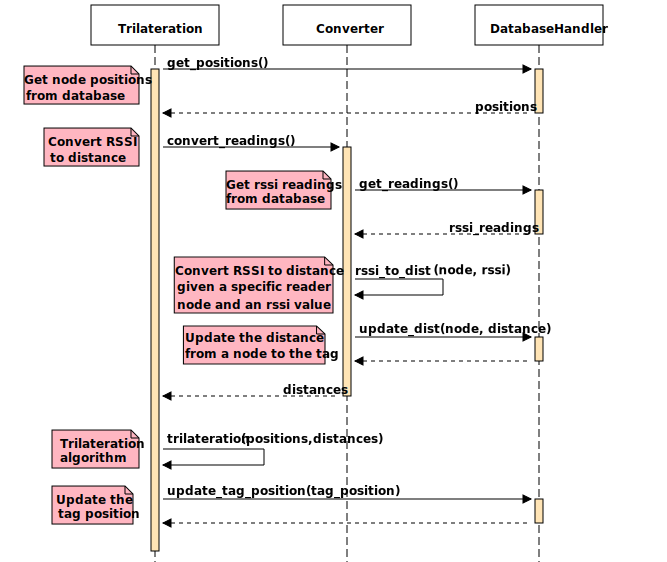
\includegraphics[width=0.55\textwidth]{figures/trilat}
		\caption{The trilateration technique for positioning an unknown node based on distance measurements from three reference nodes. Figure from \cite[p. 281]{Zhang2009}.}
		\label{fig:trilat}
	\end{center}
\end{figure}


\subsection{Evaluating an estimated position}

An important requirement for every location system is to estimate positions consistently and accurately. Hightower \cite{Hightower2001c} proposed criteria for the classification of such systems based on properties including accuracy, precision, and distribution of erroneous positions to the true one. Such metrics can be used when evaluating a location system's performance in terms of how often it locates an object within some distance of its true location. For instance, if a GPS receiver can locate its position within five meters for 90 percent of the time, then its accuracy is five meters and has a precision of 90 percent for that accuracy \cite{Hightower2001}. There is a trade-off between accuracy and precision. To achieve a higher precision, one might have to sacrifice accuracy. As a result, in order to arrive at a concise quantitative summary of these attributes, Hightower proposed to assess the error distribution accumulated during a system's operation \cite{Hightower2001}. In addition, this should be combined with other parameters such as the number of nodes in the system, the density of the infrastructure, and the size of the indoor space. In this work, these metrics are used to evaluate the localisation performance of the resulting system.

\section{Previous work}
\label{sec:prevwork}

The RFID technology is of substantial interest to researchers. Location sensing using active RFID devices is a specific subcategory of this field. Nevertheless, there have been a number of important research efforts to construct localisation systems using the available RFID hardware at that time. This section presents some of the previous work that directly relates to this project.


\subsection{SpotON}

SpotON is a fine-grained tagging technology for 3D location sensing using radio signal strength analysis \cite{Hightower2000}. The author's motivation was to develop a low cost system compared to commercial solutions available at their time. SpotON's operation involves a number of readers collecting signal strength information from active tags to determine their positions in the 3D space. It was the author's believe that the accuracy and efficiency of location sensing could be enhanced by sensor fusion, i.e. adding more sensors (accelerometers) and building proximity maps \cite{Hightower2000}.

\subsubsection{Operation}

The SpotON algorithm consists of two main parts. First, RSS measurements are converted into a distance estimation. This is done using a translation function relying on numerical variables that were identified based on observation. This function is hardware-specific and cannot be applied in this project. Second, distance measurements are used as an input to a localisation algorithm that tries to minimise RSS errors \cite{Hightower2000}. It is based on the lateration geometrical process to estimate a position for an active RFID tag.

\subsubsection{Limitations}

At the time or their research, Hightower and his colleagues were using RFID hardware with 2-bit accuracy when measuring received signal strength \cite{Hightower2000}. They identified that this accuracy is not enough to achieve the precision required for localisation in small indoor environments. The authors mentioned that 8-bit accuracy (supported by this project's hardware) could be used in the future for improved performance \cite{Hightower2000}. Another limitation was the frequency of collecting measurements. This would take between 10 and 20 seconds, which is generally too slow for monitoring real-time position changes of objects. These drawbacks were solved by creating custom RFID hardware.

\subsubsection{Results}

When localising a tagged object, the SpotON system achieved accuracy of three meters using off-the-self hardware \cite{Hightower2000}. Relying on their custom RFID devices, SpotON reported under one meter location sensing accuracy.


\subsection{LANDMARC}

LANDMARC is a 2D location sensing system that uses RFID for locating objects inside buildings. The major advantage is that it improves the overall accuracy of locating objects by using reference tags \cite{Ni2004}. The authors believed that the choice of technology and techniques is of crucial importance for the granularity and accuracy of the location information. They identified that the range of an RFID system is determined by the power available at the tags, indoor topology, and environmental conditions. Ni and his colleagues found out that instead of using a lot of readers, they can arrange a number of tags in a 2D rectangular grid to use as reference tags \cite{Ni2004}. The advantage is that tags are cheaper than readers. Also, reference tags are subject to the same environmental factors as the tags being tracked. The authors argue that the placement of readers and reference tags is very important for the accuracy of the system \cite{Ni2004}.

\subsubsection{Operation}

The core idea of LANDMARC is to select the k nearest reference tags that are closest to the unknown tag using differences in RSS measurements. Having identified the k nearest reference tags, their known positions are used to localise the unknown tag. Distances between tags are computed using Euclidean distance. The system also applies a weighing factor when computing coordinates, where small distances receive a bigger weight.

\subsubsection{Limitations}

The hardware problems of the current RFID technology were identified \cite{Ni2004}. RFID hardware used in LANDMARC did not supply signal strength directly, which resulted in unnecessary processing and sacrificed accuracy. LANDMARC took a substantial time to estimate locations. Two factors were contributing to these problems. One being the scanning time of the readers in order to collect signal strengths. The second, the time interval of a tag emitting its identification information, which could not be controlled. Ni and his colleagues also measured different power levels from two tags placed at identical positions. This resulted in unstable system behaviour.

\subsubsection{Results}

The authors experimented with different number and placement of readers, reference and tracking tags. The best setup was consisting of four readers and one reference tag per square meter resulting in an average distance error of one meter \cite{Ni2004}.

\subsubsection{Extension systems}

VIRE extends the methods used in LANDMARC by defining virtual reference tags and a proximity map that every reader records \cite{Zhao2007}. This proximity map consists of a 2D grid of reference tags where the centre of a cell is a tag. The difference in the RSS measurements between reference and unknown tag helps label cells in the proximity map so that it can be constructed. The union of individual proximity maps gives a global proximity map for the unknown tag. Experimental results showed an improvement of LANDMARC's precision between 17 and 73 percent for different scenarios and indoor environments \cite{Zhao2007}.

LANDMARC is a location sensing system that reports a two dimensional tag positions. The extended 3-D LANDMARC algorithm is a system that could localise tags in three dimensions \cite{Khan2009}. A major difference is the use of passive tags instead of active ones. This system solves some of the original limitations of LANDMARC by using hardware providing received signal strength directly. The authors rely on similar methodology, but extend computations to three dimensions. The accuracy of the system was estimated at around 0.5 meters when employing three readers, two tracking tags, and 11 reference tags in an 11 cubic meter space \cite{Khan2009}.


\section{Summary}

This chapter presented background information of the technologies and hardware used in this project. First, an introduction of RFID is provided in Section \ref{sec:rfid}.  Then, Section \ref{sec:rssi} discusses the Received Signal Strength Indicator (RSSI). Next, the hardware components of the project are described in Section \ref{sec:projhard}. Section \ref{sec:locsens} includes a discussion of location sensing techniques and evaluation criteria. This chapter is concluded by a survey of previous work relating to this project.

\chapter{Methodology}
\label{ch:methodology}

This project explores the possibility of developing an RFID location sensing system using cost-effective hardware. This chapter details the software engineering tools and mathematical techniques that were employed to achieve this goal.

\section{Project management}

A number of considerations were taken into account when deciding how to manage this project. First, the system operates using a server-client model. This means that different software components are executing on multiple processing nodes. As a result, changes in one node need to be propagated in the whole system ensuring the consistency of the software.  Second, the software implementation is making use of different programming languages, multiple programming libraries, and a database management system. In order to ensure an iterative development process, where software components are constructed, debugged, and packaged together, it was decided to use the \textsc{Git} version control system\footnote{\textsc{Git} version control system - \url{http://git-scm.com/}}. This system keeps a distributed repository of all software and database files so that each node stores a copy of not only the whole software system, but also a complete history of changes. In addition, the use of a version control system stimulates the developer to merge a number of important changes into versions of the software. In this way, it becomes easy to track and monitor the project progress. The source code and documentation were hosted in a private repository on \textsc{GitHub}\footnote{The private project repository - \url{https://github.com/sandio/raspi-rfid-tracking}} with access granted to the people involved in developing and supervising the project.


\section{Software Engineering Practices}

A number of software engineering practices were of significant help when developing the RFID location sensing system. This section presents them and explains the problems that they solve.  

\subsection{Project decomposition}

It would have been a serious challenge to approach the project's task directly. The system consists of pieces of hardware that had to be orchestrated to solve a common problem. Therefore, it was very important to identify the system's components from early on. Hierarchical relationships between these parts were also defined. These steps ensured that the project could be divided into stages in order to systematically solve the main task. Regular deliveries of working components provided a more manageable way of constructing the final solution. For example, the work plan, devised before the start of the project, consisted of the following key activities:

\begin{enumerate}
 	\item Prepare the single-board computers
 	\item Construct functional RFID reader nodes
 	\item Receive information from the active RFID tag
 	\item Establish a network communication between nodes
 	\item Develop the localisation algorithm
 \end{enumerate}

Iterative construction of the system aided the development process. Problems and challenges were appearing gradually which helped solving them one at a time. 

\subsection{Object-oriented design}

This location sensing system is a combination of different software technologies. For instance, the system required an interface between a single-board computer and an RFID receiver. It also required means of communication between processing nodes. Logically, these and other requirements could be grouped into sets of functions, which is a motivation for employing an object-oriented design. This software methodology was used from the beginning of the project. Similar functionality is organised in a class. A class is responsible for all procedures concerning a particular part of the system. As a result, software is split into categories of functions, which makes it easy to address the class in charge of certain functionality.

Another benefit of the object-oriented design is modularity. For example, once input data is collected from all nodes it could be processed by a localisation algorithm in order to estimate the tag's position. Trilateration was chosen as the technique for computing locations. Object-oriented software development provides an easy way to experiment with different algorithms by substituting one class with another.

\subsection{System scalability}

In this project, three single-board computers collaborate by exchanging RFID readings to localise a tagged object. Three reference points are needed in order to use trilateration in two dimensions  \cite{Zhang2009}. Nevertheless, more reader nodes could be used, in case multileration is implemented, to give a better approximation of a tag's position. Another scenario involves nodes disconnecting and later reappearing into the network. These possible cases show the dynamic nature of the system. It could scale up as the system grows, but also scale down if a reader node is faulty. This is an important property of the system, which was noted at the start of the project. To ensure scalability of the server-client model, the multi-threading programming model was used. It allows multiple threads to exist within the context of a single process. As a result, the system could concurrently receive RFID measurements from multiple reader nodes, update data structures, and compute the location of the unknown object.

\subsection{Documentation}

Writing documentation was an important part of this project. The source code of the system has been systematically documented throughout the development process. Using the inline comments specifying how the software components work, an Application Programming Interface (API) was constructed using \textsc{Sphinx}\footnote{\textsc{Sphinx} - a Python documentation generator - \url{http://sphinx-doc.org/index.html}}, a \textsc{Python} documentation generator. The API contains specifications of data structures, variables, and functions. It is a valuable source of information that provides a quick reference of how the system's components work and interact with each other. In addition, a manual for future users of the system was written. It gives a quick introduction of how to set up and use the system. The API and user manual can be viewed in Appendix \textbf{REF}  \textbf{TODO}.

This project consists of both hardware and software components. In order to clearly understand how hardware components are connected and how software objects interact, a number of diagrams were used in Chapter \textbf{REF} and in the user manual. These diagrams were generated using \textsc{Blockdiag} \footnote{\textsc{Blockdiag} - simple diagram images generator - \url{http://blockdiag.com/en/}} , a diagram image generator written in \textsc{Python}.

\section{Converting RSSI to distance}
\label{sec:rssitodist}

One of the main challenges of this project was to find a reliable way of converting RSSI values into distance from RFID readers to a tag. As discussed in Section \ref{subsec:rsssianddist}, studies have shown that RSSI is not a reliable or accurate measure of distance. Nevertheless, RSSI is one of the main parameters of this system and distance estimation is solely based on it.

\subsection{Free-space Path Loss}

The first attempt to provide a conversion between RSSI and distance was relying on the inverse-square physical law and free-space path loss (FSPL) formula. In free space propagation, electromagnetic waves obey the inverse-square law stating that the intensity of the emitted radiation is inversely proportional to the square of the distance from the source of the emitted radiation \cite[p. 19]{Schlaikjer1962}. This can be expressed as the following relation:

\[ Intensity \propto \frac{1}{distance^{2}} \]

A more complete relationship between signal strength and distance is given by the FSPL formulation. Free-space path loss is the loss in signal strength of an electromagnetic wave propagating through free space without any obstacles \cite{Balanis2012}. FSPL is proportional to the square of both distance and frequency of the radio signal. It can be expressed in terms of decibels given distance in meters and radio frequency in megahertz\footnote{Derivation the dB version of the FSPL equation - \url{http://www.ece.uvic.ca/~peterd/35001/ass1a/node1.html}}: 

\[ FSPL(dB) = 20\log_{10}(d_{meters}) + 20\log_{10}(f_{MHz}) - 27.55 \]
	
Rearranging the terms of the equation to find the distance gives:

\[ d_{meters} = 10^{(FSPL(dB) - 20\log_{10}(f_{MHz}) + 27.55) / 20} \]

Section \ref{subsec:rssiandrss} discussed the relationship between RSSI and received signal strength (RSS). RSSI is a unitless measurement derived from the values of the RSS. In Section \ref{subsec:receiver}, Figure \ref{fig:rssi} shows the relationship between RSSI and RSS for the RFID receivers used in this project. Consequently, RSSI values can be converted to received signal strength expressed in $dBm$ and inserted into the equation above as $FSPL(dB)$. The frequency of the RFID project hardware is  $315MHz$ (see Table \ref{tbl:reader} and \ref{tbl:tag}).

There are three problems with this approach. First, it models how the signal strength decreases in a line-of-sight propagation in a free from obstacles environments. This project is concerned with location sensing in indoor spaces making the free-space path loss formula inappropriate for this setting. Second, computing the distance for the minimum ($0dB$) and maximum ($60dB$) values of the signal strength range results in distances $0.075$ and $75.716$ meters, which is beyond the practical range of the RFID devices. Third, the conversion from RSSI to RSS might not be appropriate in this case. The RFID equipment for this project is more affordable compared to commercial RFID equipment\footnote{How much do RFID readers cost today? - \url{http://www.rfidjournal.com/faq/show?86}}. As a result, the online support and specifications are scarce, which raises the question to what extent these can be trusted. Moreover, the manufacturer claims a RSSI resolution of eight bits outputting values between 0 and 255. During the range experiments with this hardware a much smaller resolution was recorded. Consequently, converting RSSI unitless values to received signal strength in $dBm$ cannot be relied upon. For details on the evaluation of the RFID devices refer to \textbf{REF}. 

\subsection{Translation table}

Rather than relying on the physical relationship between electromagnetic waves and distance, a simpler and more direct approach was taken. For each RFID reader, a translation table was constructed mapping RSSI to distance. According to the manufacturer, but also observed in hardware experiments, reader measurements vary between different devices. There are two reasons for this. First, the RFID readers are handmade, which introduces small differences in their circuits. Second, the devices are not calibrated to each other when being built.   

The methodology for constructing these translation tables relies entirely on RSSI measurements collected while evaluating the RFID devices. A number of experiments were conducted testing how RSSI changes as the distance between a reader and tag increases. In order to account for the characteristics of indoor environments, these experiments have taken into account the orientation of the tag to the reader, line-of-sight propagation versus obscuring the tag with an obstacle, and elevation of the tag to the reader. Combining measurements from different experiments gives a more realistic representation of how RSSI changes in an indoor environment. Table \ref{tbl:trans} presents the translation table constructed for the first reader. Similar tables were developed for the other two devices (see Appendix \ref{sec:trans}).

\begin{table}[h]
	\centering
	\begin{tabular}{ | c | c | c || c | c || c | c || c | c || c | c || c | c || c | c | }
		\hline
		Distance 	& 0  & 1  & 1  & 2  & 2  & 3  & 3  & 4  & 4  & 5  & 5  & 6  & 6  & 7  \\ \hline
		RSSI 		& 80 & 65 & 64 & 62 & 61 & 57 & 56 & 53 & 52 & 48 & 47 & 46 & 45 & 44  \\ \hline
	\end{tabular}
	\caption{RSSI value ranges used to estimate distance when using the first reader.}
	\label{tbl:trans}
\end{table}

As an example, the first two columns of Table \ref{tbl:trans} have the following meaning. When the reader and tag antennas were touching the average RSSI value from all experiments was 80. When the tag was one meter away from the reader, the average RSSI value of all experiment measurements was 65. RSSI values between 80 and 65 are linearly converted to the new range from zero to one meters as follows: 

\[Old.range = old.min - old.max \\\]
\[New.value = new.min + (old.min - old.value) / old.range\]

An obvious limitation of these conversions is the size of the RSSI ranges. For example, there are 15 possible values that the first reader could measure when the tag is between zero and one meters away from it. In contrast, for a distance between six and seven meters the RSSI values change only by one unit. Following from that, the granularity of the distance estimation changes depending on the range of the RSSI measurements. This is caused by a hardware limitation of the readers when measuring RSSI and has been found during the range experiments presented in \textbf{REF}.

There is another factor contributing to the accuracy of this conversion. The RFID tag is using a battery for its power supply. During continuous operation the battery power level gradually drops, thus the tag emits a weaker radio signal as the battery is being depleted. This is reflected in the RSSI measurements making the translation tables inaccurate. In order to account for the RSSI changes, the incoming measurements were increased by an integer factor chosen based on observation. Different factors were selected for each reader due to their measurement differences.

In summary, this conversion method is not universal and probably cannot be applied to other brands of RFID devices. There are numerous factors that contribute to the variations in RSSI such as radio signal reflection, multi-path fading, and shadowing, to name a few. Nevertheless, this method was selected to translate RSSI to distance. Once the translation tables are constructed, it is a matter of calibration. As mentioned above, RSSI to distance conversion is one of the main variables of this system. How these translation tables performed is discussed in Section \textbf{REF}, where the evaluation results of the system in terms of localisation accuracy are presented.


\section{Trilateration}
\label{sec:trilatmeth}

Trilateration is a localisation method computing the position of an unknown object based on range measurements from three reference points at known locations. The concept of this technique was described in Section \ref{sec:trilatback}. This section presents the mathematical technique used in this project that provides an exact and computationally efficient solution for three-dimensional position estimation. The solution is based on the work of Manolakis \cite{Manolakis1996} and the Wikipedia article on trilateration \cite{Wikipedi2013}.

\subsection{Special case}

In three-dimensional Cartesian coordinate system, the equations for three spheres are:
\begin{align*}
	r_1^2 &=(x-x_1)^2+(y-y_1)^2+(z-z_1)^2 \\
	r_2^2 &=(x-x_2)^2+(y-y_2)^2+(z-z_2)^2 \\
	r_3^2 &=(x-x_3)^2+(y-y_3)^2+(z-z_3)^2 \\
\end{align*}
where the sphere centres are $\vec p_1 = (x_1, y_1, z_1), \ \vec p_2 = (x_2, y_2, z_2), \ \vec p_3 = (x_3, y_3, z_3)$ and $r_1$, $r_2$, and $r_3$ are the sphere radii. Solving these equations for $x$, $y$, and $z$ would give their intersection point. However, this is hard to do directly. In order to simplify the calculations, a special case is defined that later can be used as the basis for a general solution. There are three requirements of the special case. First, the three centres of the spheres are on the $z=0$ plane, hence working in two dimensions. Second, one of the centres of the spheres, $\vec p_1$, is located at the origin. Third, another centres of the spheres, $\vec p_2$, is on the $x$-axis, thus two of the spheres are collinear. The equations for the three spheres can be rewritten as follows:
\begin{align}
	r_1^2 & =x^2+y^2+z^2 \label{eq:1}\\
	r_2^2 & =(x-d)^2+y^2+z^2 \label{eq:2}\\
	r_3^2 & =(x-i)^2+(y-j)^2+z^2 \label{eq:3}
\end{align}
where $d$ is the distance between sphere centres $\vec p_1$ and $\vec p_2$ and $i$ and $j$ are the signed magnitudes of the $x$ and $y$ components of the vector from $\vec p_1$ to $\vec p_3$. Figure \ref{fig:trilat2} illustrates these components and the positions of the spheres in the $z=0$ plane.

To solve these equations, first subtract \ref{eq:2} from \ref{eq:1} and solve for $x$:
\[x=\frac{r_1^2-r_2^2+d^2}{2d}\]
Next, subtract \ref{eq:3} from \ref{eq:1} and solve for $y$:
\[y=\frac{r_1^2-r_3^2+i^2+j^2}{2j}-\frac{i}{j}x\]
Finally, use \ref{eq:1} to solve for $z$:
\[z=\pm \sqrt{r_1^2-x^2-y^2}\]
These three equations  provide the coordinates of the intersection point $(x,y,z)$ of the three spheres.

\begin{figure}[h]
	\begin{center}
		\def\svgwidth{0.6\textwidth}
		\input{figures/trilat2.pdf_tex}
		\caption{Figure showing three intersecting spheres in the plane containing their centres. Figure from \cite{Wikipedi2013}.}
		\label{fig:trilat2}
	\end{center}
\end{figure}

\subsection{General solution}

The solution of the aforementioned case cannot be applied in a general three-dimensional case because its requirements are not met. This is overcome by treating the sphere centres, $\vec p_1$, $\vec p_2$, and $\vec p_3$, as vectors from the origin:
\begin{align*}
	\vec p_1 &= (x_1, y_1, z_1) \\
	\vec p_2 &= (x_2, y_2, z_2) = \vec p_1 + \hat e_x d \\
	\vec p_3 &= (x_3, y_3, z_3) = \vec p_1 + \hat e_x i + \hat e_y j \\
\end{align*}
where $\hat e_x$, $\hat e_y$, and $\hat e_z$ are the basis unit vectors in the $x$, $y$, and $z$ original coordinate system; $d$, $i$, and $j$ are the same variables defined above. The unit vectors and variables are expressed as follows:
\begin{align*}
	& d = \| \vec p_2 - \vec p_1 \|, &&  i = \hat e_x \cdot ( \vec p_3 - \vec p_1 ), && j = \hat e_y \cdot ( \vec p_3 - \vec p_1 ) \\
	& \hat e_x = \frac{ \vec p_2 - \vec p_1 }{ d }, && \hat e_y = \frac{ \vec p_3 - \vec p_1 - \hat e_x i}{ \| \vec p_3 - \vec p_1 - \hat e_x i \| }, && \hat e_z = \hat e_x \times \hat e_y
\end{align*}
Thus, the intersection point of the three spheres, which is the solution of the problem, is:
\[\vec p_{1,2} = \vec p_1 \ + \ \hat e_x x \ + \ \hat e_y y \ \pm \hat e_z z\]

This mathematical method is used to estimate the position of an RFID tag. It is efficient because trigonometric functions are not used. Instead, this method relies on elementary arithmetic operations \cite{Manolakis1996}. When implementing this method, one needs to account for some specific cases, for instance, when $d$ equals $0$. In this case, the sphere centres $\vec p_1$ and $\vec p_2$ share the same coordinates, which means that these two spheres are concentric. Consequently, no solution to the problem exists because these spheres cannot intersect when they have different radii and are the same sphere if they have equal radii. Section \textbf{REF} is concerned with the implementation details and conditions guarding for specific cases. 

\chapter{Design}
\label{ch:design}

This chapter details the hardware and software design of the system. Section \ref{sec:harddes} describes how the hardware devices are connected to build the system. Section \ref{sec:softdes} presents the software specifications, overall architecture, and individual components of the system.

\section{Hardware design}
\label{sec:harddes}

\begin{figure}
	\begin{center}
		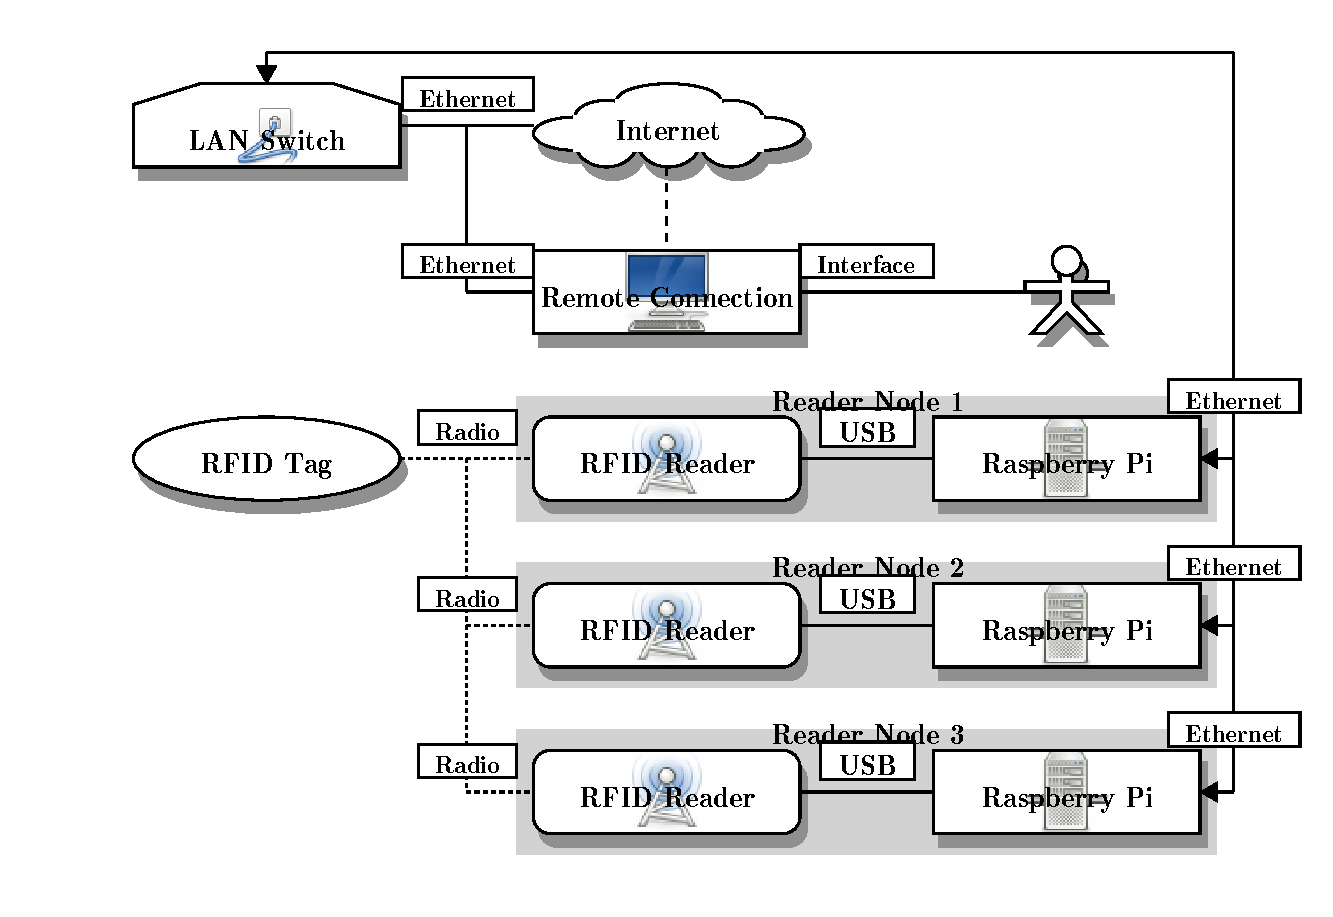
\includegraphics[width=1\textwidth]{figures/blockdiag/hardwaredesign}
		\caption{Hardware.}
		\label{fig:harddes}
	\end{center}
\end{figure}

\begin{figure}
	\begin{center}
		\includegraphics[width=1\textwidth]{figures/blockdiag/hardwaredesignwifi}
		\caption{Hardware Wifi.}
		\label{fig:harddeswifi}
	\end{center}
\end{figure}

\subsection{Antenna Design}

\section{Software design}
\label{sec:softdes}


\section{Summary}

\chapter{Implementation}
\label{ch:implementation}

This chapter details the hardware and software design of the system. Section \ref{sec:harddes} describes how the hardware devices are connected to build the system. Section \ref{sec:softdes} presents the software specifications, overall architecture, and individual components of the system.

This project explores the possibility of developing an RFID location sensing system using cost-effective hardware. This chapter details the software engineering tools and mathematical techniques that were employed to achieve this goal.



\section{Antenna Design}
\label{sec:antdes}

\section{Project management}

A number of considerations were taken into account when deciding how to manage this project. First, the system operates using a server-client model. This means that different software components are executing on multiple processing nodes. As a result, changes in one node need to be propagated in the whole system ensuring the consistency of the software.  Second, the software implementation is making use of different programming languages, multiple programming libraries, and a database management system. In order to ensure an iterative development process, where software components are constructed, debugged, and packaged together, it was decided to use the \textsc{Git} version control system\footnote{\textsc{Git} version control system - \url{http://git-scm.com/}}. This system keeps a distributed repository of all software and database files so that each node stores a copy of not only the whole software system, but also a complete history of changes. In addition, the use of a version control system stimulates the developer to merge a number of important changes into versions of the software. In this way, it becomes easy to track and monitor the project progress. The source code and documentation were hosted in a private repository on \textsc{GitHub}\footnote{The private project repository - \url{https://github.com/sandio/raspi-rfid-tracking}} with access granted to the people involved in developing and supervising the project.


\section{Software Engineering Practices}

A number of software engineering practices were of significant help when developing the RFID location sensing system. This section presents them and explains the problems that they solve.  

\subsection{Project decomposition}

It would have been a serious challenge to approach the project's task directly. The system consists of pieces of hardware that had to be orchestrated to solve a common problem. Therefore, it was very important to identify the system's components from early on. Hierarchical relationships between these parts were also defined. These steps ensured that the project could be divided into stages in order to systematically solve the main task. Regular deliveries of working components provided a more manageable way of constructing the final solution. For example, the work plan, devised before the start of the project, consisted of the following key activities:

\begin{enumerate}
 	\item Prepare the single-board computers
 	\item Construct functional RFID reader nodes
 	\item Receive information from the active RFID tag
 	\item Establish a network communication between nodes
 	\item Develop the localisation algorithm
 \end{enumerate}

Iterative construction of the system aided the development process. Problems and challenges were appearing gradually which helped solving them one at a time. 

\subsection{Object-oriented design}

This location sensing system is a combination of different software technologies. For instance, the system required an interface between a single-board computer and an RFID receiver. It also required means of communication between processing nodes. Logically, these and other requirements could be grouped into sets of functions, which is a motivation for employing an object-oriented design. This software methodology was used from the beginning of the project. Similar functionality is organised in a class. A class is responsible for all procedures concerning a particular part of the system. As a result, software is split into categories of functions, which makes it easy to address the class in charge of certain functionality.

Another benefit of the object-oriented design is modularity. For example, once input data is collected from all nodes it could be processed by a localisation algorithm in order to estimate the tag's position. Trilateration was chosen as the technique for computing locations. Object-oriented software development provides an easy way to experiment with different algorithms by substituting one class with another.

\subsection{System scalability}

In this project, three single-board computers collaborate by exchanging RFID readings to localise a tagged object. Three reference points are needed in order to use trilateration in two dimensions  \cite{Zhang2009}. Nevertheless, more reader nodes could be used, in case multileration is implemented, to give a better approximation of a tag's position. Another scenario involves nodes disconnecting and later reappearing into the network. These possible cases show the dynamic nature of the system. It could scale up as the system grows, but also scale down if a reader node is faulty. This is an important property of the system, which was noted at the start of the project. To ensure scalability of the server-client model, the multi-threading programming model was used. It allows multiple threads to exist within the context of a single process. As a result, the system could concurrently receive RFID measurements from multiple reader nodes, update data structures, and compute the location of the unknown object.

\subsection{Documentation}

Writing documentation was an important part of this project. The source code of the system has been systematically documented throughout the development process. Using the inline comments specifying how the software components work, an Application Programming Interface (API) was constructed using \textsc{Sphinx}\footnote{\textsc{Sphinx} - a Python documentation generator - \url{http://sphinx-doc.org/index.html}}, a \textsc{Python} documentation generator. The API contains specifications of data structures, variables, and functions. It is a valuable source of information that provides a quick reference of how the system's components work and interact with each other. In addition, a manual for future users of the system was written. It gives a quick introduction of how to set up and use the system. The API and user manual can be viewed in Appendix \textbf{REF}  \textbf{TODO}.

This project consists of both hardware and software components. In order to clearly understand how hardware components are connected and how software objects interact, a number of diagrams were used in Chapter \textbf{REF} and in the user manual. These diagrams were generated using \textsc{Blockdiag} \footnote{\textsc{Blockdiag} - simple diagram images generator - \url{http://blockdiag.com/en/}} , a diagram image generator written in \textsc{Python}.

\section{Summary}

\chapter{Evaluation}
\label{ch:evaluation}

This chapter describes the experiments conducted to evaluate the RFID hardware and localisation accuracy of the system. Each experiment description consists of justification, setup, results, and analysis. Section \ref{sec:hardeval} presents tests of the RFID hardware that provide an understanding of the mapping between RSSI and distance. Then, section \ref{sec:syseval} details the experiments that check whether the problem, described in section \ref{sec:probdef}, is solved by the system. It also provides results in terms of localisation accuracy and how these compare to results of the related work.

\section{Hardware Evaluation}
\label{sec:hardeval}

This section presents the experiments conducted in attempt to correlate received signal strength indicator (RSSI) and distance. This was accomplished by positioning the RFID tag at increasing distances and recording RSSI measurements from the RFID readers. Distance measurements were marked by a tape measure and RSSI values were recorded using the \textsf{SerialConnection} class developed as part of the system (details in section \ref{sec:constread}). All experiments had taken place in two indoor environments, an apartment and a university computer laboratory. These places differ in the amount of open space and the number and placement of objects.

In indoor environments, the attenuation of a radio signal is strongly influenced by the physical effects of reflection, refraction, multipath and shadow fading. Following from that, in order to construct a more complete notion of the relationship between RSSI and distance, a number of experiments were carried out. These include how RSSI changed as distance increased at different orientations of the tag to the readers and elevations of the tag from the floor. In addition, the wall penetration and range capabilities of the hardware were evaluated. The following subsections describe these experiments.

\subsection{Range}

The aim of this experiment was to measure the range capabilities of the RFID equipment in an indoor environment. In addition, RSSI values were recorded as distance between the readers and tag increased. In the first part of the experiment, the devices were keeping a line of sight between each other. Then, the test was repeated by obscuring the tag with an object, in this case a large whiteboard, to determine if it was affecting the communication range of the devices and the RSSI values reported by the readers. The experiments were carried out for each of the readers in a computer laboratory that had a 13-meter-long stretch of open space. The results of these experiments are illustrated on Figure \ref{fig:13m}.

\begin{figure}[h]
	\begin{center}
		\includegraphics[width=1\textwidth]{figures/rssi_distance_13m}
		\caption{Two plots of RSSI measurements at increasing distances. On the $x$-axis, the distances from one to 13 meters are shown. The $y$-axis is the RSSI range. Notice how the RSSI ranges differ between the plots. The left graph shows how RSSI values measured at the three readers change with a line-of-sight signal propagation. The right graph illustrates the same experiment but with a non-line-of-sight signal propagation - the tag is occluded by an object.}
		\label{fig:13m}
	\end{center}
\end{figure}

There are three observations that could be made by looking at these results. First, in both experiments all three readers were able to detect the tag when located 13 meters away. The manufacturer reported a transmission range of 8 meters. Consequently, the antenna, designed in this project, had definitely increased the transmission range of the RFID tag. 

Second, these experiments confirm that the readers measure different RSSI for the same distance. As distance increases, the average difference between RSSI values is 4.93. The ranges on the $y$-axis are between 20 and 30 RSSI. Following from that, if the measurements reported by the readers differ in an average of around five units given the above ranges, then these readers are not calibrated to each other. This was observed in subsequent experiments as well. It was the motivation for constructing separate translation tables when mapping RSSI to distance.

Third, it is known that radio signals suffer from the effects of various physical phenomena when propagating in indoor environments. This was seen in all experiments when evaluating the RFID devices. Figure \ref{fig:13m} clearly shows that RSSI measurements do not decrease steadily and often fluctuate as the distance increases. This could be contributed to the characteristics of indoor spaces, where the shape of the space and the objects in it could cause reflection, refraction, and absorption of radio signals. Introducing an object that occluded the RFID tag had definitely decreased the RSSI values reported by the readers. It also caused the measurements to vary in unexpected ways.

\subsection{Line-of-sight Grid RSSI}

\begin{figure}[H]
	\begin{center}
		\includegraphics[width=1\textwidth]{figures/rssi_distance_grid_r1}
		\caption{Sixteen plots are organised into a four by four grid. Each plot represents the RSSI measurements of the \textbf{first} reader when the tag is placed at different positions on the x and y axes of the grid. The positions of the tag are all measured in meters. Every four bars in each plot show the RSSI readings when the tag is facing right (0\textdegree), up(90\textdegree), left (180\textdegree), and down (270\textdegree).}
	\end{center}
\end{figure}

\subsection{Orientation of tag to reader}

Conducted an experiment with the 3 readers and the active tag. Goal: to observe how the RSSI is changing as the tag moves away from a reader. Experimental setup: For every reader the tag is placed next to it, then 0.5m, 1m, 1.5m, 2m, 2.5m, and 3m away from the reader. For every distance the RSSI is recorded when there is a direct line of sight between the reader and the tag but also when the direct line of sight is obscured by some object (a suitcase filled with stuff). This is done for every reader and for every orientation of the reader (0, 45, 90, 135, 180, 225, 270, 315) to see if the readings get affected by the orientation of the reader. As a result, we get 8 tables (1 for every orientation) consisting of readings from the 3 readers once with a direct line of sight and once with an obscured line of sight (6 columns). These tables have 7 rows (1 for each distance). The results will be plotted and included in the final report where there will be a discussion of the implications of these results.

\begin{figure}[h]
	\begin{center}
		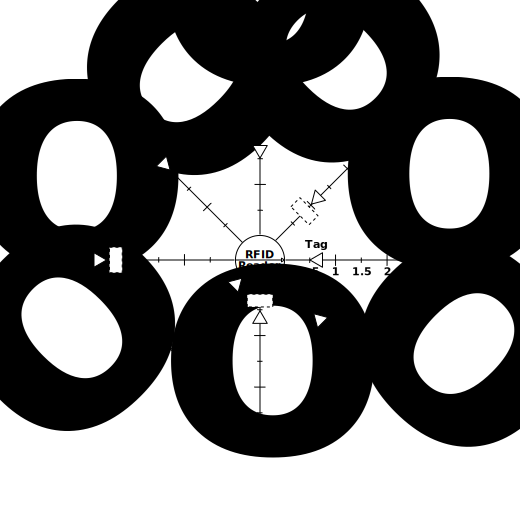
\includegraphics[width=.8\textwidth]{figures/exp/orientation}
		\caption{}
		\label{fig:ori}
	\end{center}
\end{figure}

\begin{figure}[H]
	\begin{center}
		\includegraphics[width=1\textwidth]{figures/rssi_distance_3m_0deg}
		\caption{Two plots of RSSI measurements at increasing distances with the readers at 0 degrees (antennas facing the tag). The left graph show how RSSI values change with a line-of-sight signal propagation. The right graph illustrates the same experiment but with a non-line-of-sight signal propagation (there is an obstacle between the reader and the tag).}
	\end{center}
\end{figure}



\begin{figure}[H]
	\begin{center}
		\includegraphics[width=1\textwidth]{figures/rssi_distance_3m_90deg}
		\caption{Two plots of RSSI measurements at increasing distances with the readers at 90 degrees (antennas at an angle to the tag). The left graph show how RSSI values change with a line-of-sight signal propagation. The right graph illustrates the same experiment but with a non-line-of-sight signal propagation (there is an obstacle between the reader and the tag).}
	\end{center}
\end{figure}


\subsection{Elevation}

Conducted an experiment with the 3 readers and the active tag. Goal: to measure if the position of the tag in height from the ground affects the RSSI. Experimental setup: The readers are positioned at floor level (6cm), at desk level (60 cm), and at 130cm. The tag is placed at the same heights at distances 1m, 1.5m, 2.0m, 2.5m, 3.0m, 3.5m, 4.0m. This results in a table with RSSI with 9 columns (3x for each reader at different heights) and 7 columns for each distance.

\begin{figure}[H]
	\begin{center}
		\includegraphics[width=1\textwidth]{figures/rssi_distance_4m}
		\caption{Three plots of RSSI measurements at increasing distances with the readers at different elevation from the floor in an indoor environment. The first graph shows how RSSI measurements change as the distance grows when the tag is placed at 6cm above floor level. The second and third graph show the same experiment but the tag is at 60cm and 130cm above the floor level.}
	\end{center}
\end{figure}


\subsection{Wall penetration}

Conducted an experiment with one reader and the active tag. Goal: to see the penetration capabilities of the tag/transmitter. Experimental setup: The reader was placed in one room, the tag in the adjacent room separated by a thin wall. The distance apart was 3m and RSSI: 41. Then I moved the tag in the next room adjacent to the previous so that the straight line between tag and reader is preserved. The tag was read at 4.8m distance with RSSI: 51. In the same room the tag was moved at the furthest possible position in the room at 8.2m with RSSI: 40. Then I got outside and went behind the building. The tag was read behind a 3rd thicker wall at distance 8.6m with RSSI: 32.

\section{System evaluation}
\label{sec:syseval}

By "mapping" I meant that the experiments check whether the problem is solved by the system, i.e. whether they give us a reliable way of checking the hypothesis. 

\subsection{Line-of-sight Grid Error}

Conducted a experiment in AT 3.01 (Robotics Lab). I took all the equipment, which fits into my backpack. I cleared a space 3 by 3 meters with no obstacles (line-of-sight propagation). Placed the reader nodes at 3 of the sides of the forming grid. Then I connected the whole system and powered it up. In this space, I placed markers every meter, thus forming a grid with 16 possible positions to place the tag. I did RSSI measurements at each position and also rotating the tag by 90 degrees. This resulted in 3 tables of RSSI measurements, one per reader. Each table consists of 16 cells, one for every position. Every cell has four RSSI values for different orientations of the tag. I also constructed a table with error measurements for every orientation of the tag. The error is a positive value in meters for both x and y axes reflecting the difference between real and estimated positions. 

\begin{figure}[H]
	\begin{center}
		\includegraphics[width=1\textwidth]{figures/error_distance_grid}
		\caption{Sixteen plots are organised into a four by four grid. The readers are placed at positions (0,0), (0,3), and (3,0). Each plot represents the error in meters between measured and estimated location when the tag is placed at different positions on the grid. Each plot consists of four ellipses that illustrate the x and y error when the tag is facing right (0\textdegree), up(90\textdegree), left (180\textdegree), and down (270\textdegree). The colours of the ellipses are red, green, blue, and black, respectively.}
	\end{center}
\end{figure}

\begin{figure}[H]
	\begin{center}
		\includegraphics[width=1\textwidth]{figures/error_boxplot}
		\caption{A box plot showing errors between measured and estimated locations. The boxes are organised in four groups. Each group consists of errors in the x and y axes for a particular orientation of the tag. The horizontal line across the plot is the mean of all errors regardless of the tag orientation.}
	\end{center}
\end{figure}

\section{Discussion}

\section{Summary}

\chapter{Discussion and Future Work}
\label{ch:discussion}

\include{future.work}
\chapter{Conclusion}
\label{ch:conclusion}

This chapter summarises the goals of this project and provides a description of its contributions. Then, section \ref{sec:future} gives ideas how to further develop and extend the location sensing system created in this project.

\section{Contribution}

The main aim of this project was to explore the possibility of developing a location sensing system using cost-effective RFID hardware and single-board computers. The system had to be able to estimate the position of an unknown object in three-dimensions with a localisation accuracy comparable to similar systems in this research field.

Such a system was successfully developed in the duration of this project. It consisted of three RFID readers connected to  Raspberry Pi computers, forming the reader nodes of the system. Communication was established using Ethernet network cables. The object that had to be localised was an RFID tag, a small transmitter operating on battery power. This system was being able to estimate the position of the tag with an average localisation error of 0.916 meters. This performance is similar to the results of the previous work in this field. This is a positive indication because the RFID hardware employed in this project had a lower price and quality compared to commercial solutions costing ten to fifteen times more \footnote{BuyRFID online store - Prices of active RFID readers - \url{http://goo.gl/XTGsLA}}.

There are some general advantages of the system developed in this project. The software was written in a modular way making it easy to change the localisation algorithm and wireless technology. For example, Bluetooth or WiFi devices can be used for location sensing. Furthermore, the system was developed with scalablility in mind, which means that more affordable computer nodes can be connected to the network to expand the system. The system's hardware is very portable and consumes little power. The reader nodes can be positioned in various places occupying little space. The Raspberry Pi computers possess substantial processing power that speed the computations performed by the localisation algorithm. This also enabled the use of threads to concurrently execute multiple tasks of the system.

\section{Future Work}
\label{sec:future}

The system developed in this project could be extended and modified in many ways. As mentioned above different wireless technologies can be used as the basis for localisation. In addition, a bigger system consisting of many reader nodes can be constructed to cover the indoor area of a building. Moreover, according to the manufacturer specifications, the receivers can simultaneously read up to 80 tags. This issue can be investigated so that equipment or personnel can be tracked on a campus, for instance. 

This project used Raspberry Pi computers as the processing units of the system. In the current implementation, most tasks are concentrated on a single computer. Future work might involve the distribution of tasks among nodes so that the resources are utilised more efficiently. Moreover, this can alleviate the single point of failure introduced by employing a server-client model.

Potential improvements of the distance and localisation estimation might be implemented in order to solve some of the current problems of the system. In dynamic environments with people and objects occluding the transmitters, the RSSI measurements reported by the RFID readers are often fluctuating and unreliable. In order to stabilise the readings, multiple RSSI values might be collected and averaged before passing them to the localisation algorithm. In addition, the batteries of tags introduced further inaccuracies in the measurements. An integer factor was added to the incoming readings to compensate for the power lost in continuous transmissions. This parameter might be automated to eliminate manual changes of its value.

\section{Summary}
This chapter presented the contributions of the project. In addition, directions for future work were given that could lead to improvements of the current system.


\appendix
\chapter{Supplementary Information}
\label{ap:appendix}

\section{Hardware setup using Wi-Fi connectivity}
\label{sec:hardsetwifi}

\begin{figure}[h]
	\begin{center}
		\includegraphics[width=1\textwidth]{figures/blockdiag/hardwaredesignwifi}
		\caption{Hardware setup with wireless connectivity between reader nodes.}
		\label{fig:hardsetwifi}
	\end{center}
\end{figure}

\newpage
\section{Translation tables from RSSI to distance}
\label{sec:trans}

\begin{table}[h]
	\centering
	\begin{tabular}{ | c | c | c || c | c || c | c || c | c || c | c || c | c || c | c | }
		\hline
		Distance 	& 0  & 1  & 1  & 2  & 2  & 3  & 3  & 4  & 4  & 5  & 5  & 6  & 6  & 7  \\ \hline
		RSSI 		& 80 & 65 & 64 & 62 & 61 & 57 & 56 & 53 & 52 & 48 & 47 & 46 & 45 & 44  \\ \hline
	\end{tabular}
	\caption{RSSI value ranges used to estimate distance when using the first reader. }
	\label{tbl:trans1}
\end{table}

\begin{table}[h]
	\centering
	\begin{tabular}{ | c | c | c || c | c || c | c || c | c || c | c || c | c || c | c | }
		\hline
		Distance 	& 0  & 1  & 1  & 2  & 2  & 3  & 3  & 4  & 4  & 5  & 5  & 6  & 6  & 7  \\ \hline
		RSSI 		& 77 & 63 & 62 & 58 & 57 & 55 & 54 &53  & 52 & 49 & 48 & 47 & 46 & 44 \\ \hline
	\end{tabular}
	\caption{RSSI value ranges used to estimate distance when using the second reader. }
	\label{tbl:trans2}
\end{table}

\begin{table}[h]
	\centering
	\begin{tabular}{ | c | c | c || c | c || c | c || c | c || c | c || c | c || c | c | }
		\hline
		Distance 	& 0  & 1  & 1  & 2  & 2  & 3  & 3  & 4  & 4  & 5  & 5  & 6  & 6  & 7  \\ \hline
		RSSI 		& 78 & 64 & 63 & 60 & 59 & 56 & 55 & 54 & 53 & 49 & 48 & 45 & 44 & 43 \\ \hline
	\end{tabular}
	\caption{RSSI value ranges used to estimate distance when using the third reader. }
	\label{tbl:trans3}
\end{table}

\newpage
\section{Orientation}

\begin{figure}[H]
	\begin{center}
		\includegraphics[width=1\textwidth]{figures/rssi_distance_3m_45deg}
		\caption{Two plots of RSSI measurements at increasing distances with the readers at 45 degrees (antennas at an angle to the tag). The left graph show how RSSI values change with a line-of-sight signal propagation. The right graph illustrates the same experiment but with a non-line-of-sight signal propagation (there is an obstacle between the reader and the tag).}
	\end{center}
\end{figure}

\begin{figure}[H]
	\begin{center}
		\includegraphics[width=1\textwidth]{figures/rssi_distance_3m_135deg}
		\caption{Two plots of RSSI measurements at increasing distances with the readers at 135 degrees (antennas at an angle to the tag). The left graph show how RSSI values change with a line-of-sight signal propagation. The right graph illustrates the same experiment but with a non-line-of-sight signal propagation (there is an obstacle between the reader and the tag).}
	\end{center}
\end{figure}

\begin{figure}[H]
	\begin{center}
		\includegraphics[width=1\textwidth]{figures/rssi_distance_3m_180deg}
		\caption{Two plots of RSSI measurements at increasing distances with the readers at 180 degrees (antennas at an angle to the tag). The left graph show how RSSI values change with a line-of-sight signal propagation. The right graph illustrates the same experiment but with a non-line-of-sight signal propagation (there is an obstacle between the reader and the tag).}
	\end{center}
\end{figure}

\begin{figure}[H]
	\begin{center}
		\includegraphics[width=1\textwidth]{figures/rssi_distance_3m_225deg}
		\caption{Two plots of RSSI measurements at increasing distances with the readers at 225 degrees (antennas at an angle to the tag). The left graph show how RSSI values change with a line-of-sight signal propagation. The right graph illustrates the same experiment but with a non-line-of-sight signal propagation (there is an obstacle between the reader and the tag).}
	\end{center}
\end{figure}

\begin{figure}[H]
	\begin{center}
		\includegraphics[width=1\textwidth]{figures/rssi_distance_3m_270deg}
		\caption{Two plots of RSSI measurements at increasing distances with the readers at 270 degrees (antennas at an angle to the tag). The left graph show how RSSI values change with a line-of-sight signal propagation. The right graph illustrates the same experiment but with a non-line-of-sight signal propagation (there is an obstacle between the reader and the tag).}
	\end{center}
\end{figure}

\begin{figure}[H]
	\begin{center}
		\includegraphics[width=1\textwidth]{figures/rssi_distance_3m_315deg}
		\caption{Two plots of RSSI measurements at increasing distances with the readers at 315 degrees (antennas at an angle to the tag). The left graph show how RSSI values change with a line-of-sight signal propagation. The right graph illustrates the same experiment but with a non-line-of-sight signal propagation (there is an obstacle between the reader and the tag).}
	\end{center}
\end{figure}

\newpage
\section{Grid}

\begin{figure}[H]
	\begin{center}
		\includegraphics[width=1\textwidth]{figures/rssi_distance_grid_r2}
		\caption{Sixteen plots are organised into a four by four grid. Each plot represents the RSSI measurements of the \textbf{second} reader when the tag is placed at different positions on the x and y axes of the grid. The positions of the tag are all measured in meters. Every four bars in each plot show the RSSI readings when the tag is facing right (0\textdegree), up(90\textdegree), left (180\textdegree), and down (270\textdegree).}
	\end{center}
\end{figure}

\begin{figure}[H]
	\begin{center}
		\includegraphics[width=1\textwidth]{figures/rssi_distance_grid_r3}
		\caption{Sixteen plots are organised into a four by four grid. Each plot represents the RSSI measurements of the \textbf{third} reader when the tag is placed at different positions on the x and y axes of the grid. The positions of the tag are all measured in meters. Every four bars in each plot show the RSSI readings when the tag is facing right (0\textdegree), up(90\textdegree), left (180\textdegree), and down (270\textdegree).}
	\end{center}
\end{figure}


\bibliographystyle{apalike}
\bibliography{../library}

\end{document}
